\section{Etiquetado y comentarios}

Como parte de la administración de incidencias, se agregó una etiqueta para clasificar el problema como un error del sistema y tambien se añadió un comentario para indicar el inicio del seguimiento de la incidencia

Estas acciones permiten mantener un seguimiento adecuado del estado de la incidencia y facilitan la comunicación entre los integrantes del equipo.

\begin{figure}[H]
\centering
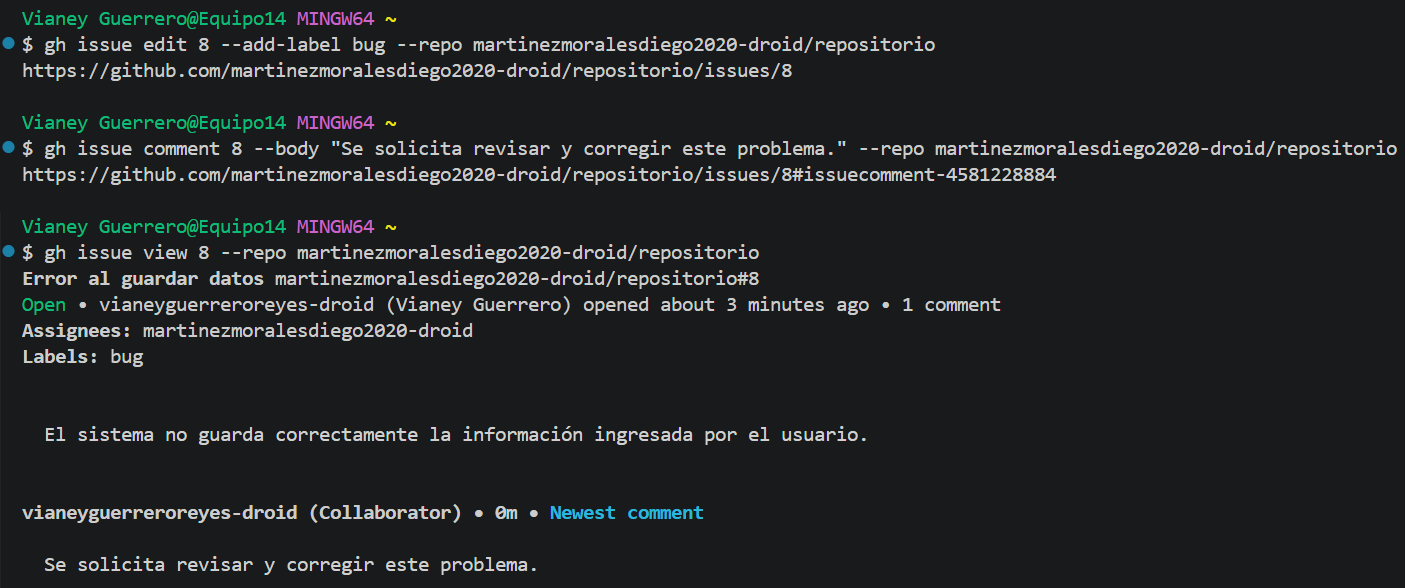
\includegraphics[width=0.9\textwidth]{M10.png}
\caption{Issue actualizado con etiqueta y comentario de seguimiento.}
\end{figure}